\documentclass[11pt,a4paper]{article}

\usepackage[margin=2.3cm]{geometry}
\usepackage{amsmath,amssymb,amsthm}
\usepackage{booktabs}
\usepackage{graphicx}
\usepackage{xcolor}
\usepackage{enumitem}
\usepackage{listings}
\PassOptionsToPackage{hyphens}{url}
\usepackage[hidelinks]{hyperref}

\lstset{basicstyle=\ttfamily\small,columns=fullflexible,breaklines=true,frame=single,
        keywordstyle=\color{blue!60!black},commentstyle=\color{gray},language=Python}

\newcommand{\file}{\nolinkurl}  % file paths: may break after / . _
\newcommand{\code}[1]{\texttt{#1}}
\newcommand{\stagepending}[1]{\begin{center}\fbox{\parbox{0.9\linewidth}{\centering\itshape
  This section is written in Stage #1, after its code exists.}}\end{center}}

\emergencystretch=3em
\newtheorem{definition}{Definition}
\theoremstyle{remark}
\newtheorem*{why}{Why}

\title{Trace-Aware POMCP for Ad Hoc Teamwork\\[2pt]
\large Method, implementation and experiments (branch \texttt{urop1020})}
\author{Minh Hien}
\date{20 November 2026 (Stages 1--6)}

\begin{document}
\maketitle

\begin{abstract}
An ad hoc agent joins a team whose members leave \emph{traces} in the environment: marks that record where they were,
whether they failed to lift a task, and in which direction they were heading. The agent does not know its teammates'
algorithms. This document explains, from the ground up, how the POMCP planner can use such traces: what is implemented,
in which file, and the mathematics behind every rule. Traces only help a planner if they change its \emph{belief} about
what it cannot see. We therefore compare a planner that ignores traces with one whose belief reads them using their true
meaning (the ``teacher'', or ``native speaker''). The next step replaces the true meaning with a \emph{learned} one.
\end{abstract}

\tableofcontents

%=====================================================================================================================
\section{Problem setting}
\label{sec:setting}
%=====================================================================================================================

\subsection{The world: Level-Based Foraging}

The environment is the Level-Based Foraging (LBF) world of the AdLeap-MAS framework (\file{src/envs/LevelForagingEnv.py},
not modified by this project). Our scenarios are built by \code{make\_scenario} (\file{src/utils/scenarios.py}) and
\code{create\_evaluation\_set} (\file{src/utils/evaluation.py}):

\begin{itemize}[nosep]
  \item a grid of $10\times 10$ cells; a cell is a pair $(x,y)$ with $x,y\in\{0,\dots,9\}$; moving \emph{East} increases
        $x$, moving \emph{North} increases $y$ (\code{new\_position\_given\_action});
  \item the \textbf{ad hoc agent} (index \code{A}): level $0.9$, view radius $0.25$, view angle $1.0$ (full circle);
  \item $2$ \textbf{teammates} (\code{w1}, \code{w2}): type \code{l1} or \code{l2} (hand-written heuristics from the
        framework, \file{src/reasoning/levelbased/}), level, view radius and view angle each drawn from $U(0.5,1.0)$;
  \item $5$ \textbf{tasks}: never on a border cell, never 4-adjacent to another task (generator rule), level drawn from
        $U(0.3,1.5)$ (the ``hard'' set, so that some tasks need two agents);
  \item actions $\{0,1,2,3,4\} = \{\text{East},\text{West},\text{North},\text{South},\text{Load}\}$.
\end{itemize}

\paragraph{Loading.} A task at cell $p$ is completed in a step when the agents that press \emph{Load} while standing next
to $p$ and facing it have levels summing to at least the task's level:
\begin{equation}
  \sum_{i\,\in\,\text{loaders}(p)} \ell_i \;\ge\; \ell_{\text{task}} .
  \label{eq:load}
\end{equation}
Each completed task gives reward $1$. An episode ends when all tasks are completed, or after $200$ steps (timeout).

\paragraph{Field of view.} With grid diagonal $D=\sqrt{10^2+10^2}\approx 14.14$, an agent with radius parameter $\rho$
sees up to distance $\rho D$; for the ad hoc agent $0.25\cdot 14.14 \approx 3.54$ cells. A cell is \emph{visible} if one
of its corners lies within that distance of the centre of the agent's cell, and inside the view angle
(\code{is\_visible}, \file{LevelForagingEnv.py}; the list of visible cells is computed by \code{find\_visible\_grids},
\file{src/utils/find_visible.py}). We write $V_t$ for the set of cells visible to the ad hoc agent at step $t$.

\paragraph{What the ad hoc agent knows.} The scenarios use \code{parameter\_knowledge=True}: for a \emph{visible}
teammate the agent knows its position and level. For a \emph{visible} task it knows its position \emph{and level},
anywhere inside the view, not only when standing next to it (the framework's \code{environment\_transformation} removes
invisible tasks but keeps the level of visible ones). Tasks seen earlier stay in the agent's memory. Everything else is
\emph{hidden}: teammates outside the view, tasks never seen, and the teammates' algorithms.

\subsection{Traces}
\label{sec:traces}

Every agent leaves a trace at its own cell after every step. The trace field is implemented by \code{TraceField}
(\file{src/communication/traces.py}). It stores, for every cell $c$, six numbers (``intent'' trace mode):
\begin{center}
\begin{tabular}{lll}
\toprule
Symbol & Field & Meaning \\
\midrule
$I(c)\in[0,1]$ & \code{intensity} & how fresh the trace is ($1$ = left this step) \\
$a(c)\in[0,1]$ & \code{age} & $0.2\times$(steps since it was left) \\
$\ell(c)$ & \code{level} & level of the agent that left it \\
$h(c)\in[0,1]$ & \code{help} & level deficit of a failed load ($0$ if none) \\
$\mathbf b(c)=(b_x,b_y)$ & \code{bearing\_x}, \code{bearing\_y} & unit vector toward the emitter's target \\
\bottomrule
\end{tabular}
\end{center}
A boolean mask $E(c)$ (\code{emitter}) marks cells holding a trace that an agent \emph{emitted} itself, as opposed to a
copy spread there by diffusion.

\paragraph{Order of operations in one step} (\code{StigmergicLevelForagingEnv.step}): (1) the world moves (all agents
act); (2) \emph{decay}; (3) every agent \emph{emits}; (4) \emph{diffusion}.

\paragraph{(2) Decay} (\code{TraceField.decay}), with decay rate $\delta = 0.2$:
\begin{align}
  I(c) &\leftarrow \max\bigl(0,\; I(c) - \delta\bigr), &
  a(c) &\leftarrow \min\bigl(a(c) + 0.2,\; 1\bigr),
\end{align}
and every field of a cell is cleared (and $E(c)\leftarrow\text{false}$) once $I(c)\le 10^{-6}$. Consequently a trace
emitted $k$ steps ago (and not refreshed) has
\begin{equation}
  a = 0.2\,k, \qquad I = 1 - 0.2\,k, \qquad k\in\{0,1,2,3,4\},
  \label{eq:age-intensity}
\end{equation}
and disappears at $k=5$. Equation~\eqref{eq:age-intensity} is what lets a reader of traces recover \emph{how many steps
ago} an agent stood on a cell.

\paragraph{(3) Emission} (\code{emit\_intent\_traces} in \file{src/envs/StigmergicLevelForagingEnv.py}). For every agent
$i$ at position $p_i$, with level $\ell_i$:
\begin{align}
  h_i &= \begin{cases}
     \min\bigl(\max(\ell_{\text{task}} - \ell_i,\,0),\,1\bigr) & \text{if $i$ pressed Load facing a task that is still there,}\\
     0 & \text{otherwise;}
  \end{cases} \label{eq:help}\\
  \mathbf b_i &= \begin{cases}
     \dfrac{g_i - p_i}{\lVert g_i - p_i\rVert} & \text{if $i$ is a teammate with a target $g_i \ne p_i$,}\\[6pt]
     (0,0) & \text{for the ad hoc agent, or without a target.}
  \end{cases} \label{eq:bearing}
\end{align}
The target $g_i$ is the task position the teammate's heuristic chose (\code{bearing\_to\_target}). The trace
$(\ell_i, h_i, \mathbf b_i)$ is then written at $p_i$ by \code{TraceField.fusion}:
\begin{itemize}[nosep]
  \item if $h_i>0$, it is always written (a help signal always wins and refreshes a standing one);
  \item else, if the cell already holds a help trace ($h(p_i)>0$), nothing is written;
  \item else it is written if $I(p_i) < 1$.
\end{itemize}
Writing (\code{TraceField.emit}) sets $I=1$, $a=0$, $\ell=\ell_i$, $h=h_i$, $\mathbf b=\mathbf b_i$ and $E(p_i)=\text{true}$.

\paragraph{(4) Diffusion} (\code{TraceField.diffuse}), with diffusion rate $\sigma=0.3$. Every emitted trace ($E(c)$ and
$I(c)>0$) offers a copy to each of its four neighbours $n$. The copy carries all fields of $c$ except intensity, which is
$\sigma I(c)$. Each copy is scored as
\begin{equation}
  \text{score} = I + 2\cdot\mathbf 1[h>0],
\end{equation}
and it is written at $n$ if $n$ holds no emitted trace ($\lnot E(n)$) and its score beats the score already at $n$. Copies
never spread further. Hence a diffused copy always has intensity at most $0.3\,(1-0.2k) < 1 - 0.2k$ for the same age:
\begin{equation}
  I(c) < 1 - 0.2\,k \quad\Longrightarrow\quad \text{the trace at $c$ is a diffused copy, its emitter stood next to $c$.}
  \label{eq:diffused-test}
\end{equation}

\paragraph{Sensing.} In intent mode the ad hoc agent senses traces \emph{locally}: it reads all six fields, but only in
visible cells $c\in V_t$ (\code{local\_traces=True}; \code{dict\_to\_tensor} multiplies the trace channels by the
visibility mask). It does \emph{not} read the emitter mask $E$; equation~\eqref{eq:diffused-test} recovers that
information from intensity and age.

\paragraph{One rulebook for two worlds (Stage 1).} The emission rules~\eqref{eq:help}--\eqref{eq:bearing} used to be private
methods of the gym wrapper. They are now module-level functions, \code{emit\_intent\_traces(env, traces)} and
\code{bearing\_to\_target(env, agent)}. The real game calls them, and POMCP's imagined copies of the world
(Section~\ref{sec:planning-world}) call the same functions.
\begin{why}
The teacher of this study is ``POMCP that knows the true meaning of traces''. That claim is only true if POMCP's
imagined traces come from exactly the rules of the real game. With one shared function the two cannot drift apart. The
wrapper's behaviour is unchanged: the existing tests \file{tests/test_stigmergic_env.py} and
\file{tests/test_traces.py} still pass (32/32).
\end{why}

%=====================================================================================================================
\section{POMCP from the ground up}
\label{sec:pomcp}
%=====================================================================================================================

\subsection{The problem POMCP solves}

The ad hoc agent faces a \emph{partially observable} decision problem (a POMDP). At each step the world is in a
\emph{state} $s$: positions of all agents, positions and levels of all tasks, and all traces. The agent picks an
\emph{action} $a$, the world moves to $s'$, the agent receives a \emph{reward} $r$ (the number of tasks completed in that
step) and an \emph{observation} $o$ (what it sees). It never sees $s$ itself. The best it can do is keep a
\emph{belief}: a probability distribution $b(s)$ over the states that are consistent with everything it has observed.
It then picks the action with the highest expected discounted return
\begin{equation}
  Q(b,a) \;=\; \mathbb E\Bigl[\,\sum_{t\ge 0} \gamma^{t} r_t \;\Bigm|\; b,\; a_0=a\Bigr], \qquad \gamma = 0.95 .
  \label{eq:return}
\end{equation}
Computing~\eqref{eq:return} exactly is hopeless here: there are far too many states. POMCP (Silver and Veness, 2010)
estimates it by \emph{imagination}: it draws guesses of the state from the belief, plays many imagined futures in a
simulator, and averages their returns.

\subsection{Particles: the belief as a bag of guesses}

POMCP does not store $b$ as a formula. It stores a list of $K$ \emph{particles}, each one complete guess of the world (here
$K=100$, the framework's \code{k}). A belief such as ``teammate \code{w1} is at $(5,4)$ with probability $0.5$'' becomes
``about $50$ of the $100$ particles have \code{w1} at $(5,4)$''. A particle is produced by the world's
\code{sample\_state(agent)} method. That method is the \textbf{belief sampler}, and it is the only place where POMCP
decides what the hidden part of the world might look like. Sections~\ref{sec:observation-model} and~\ref{sec:beliefs}
are about this method.

\subsection{One decision, step by step}

\code{pomcp\_planning(env, agent)} (\file{src/reasoning/pomcp.py}, line 218) copies the world, marks the copy as a
simulation, and calls \code{POMCP.planning} (line 185):

\begin{enumerate}[leftmargin=*]
\item \textbf{Root.} The search tree alternates \emph{observation nodes} (``what I have seen so far'') and \emph{action
  nodes} (``\ldots and then I do $a$''). If a tree from the previous decision exists, \code{find\_new\_PO\_root}
  (\file{src/reasoning/node.py}, line 213) walks down to the child for the action actually taken and the observation
  actually received, and reuses it (\emph{tree reuse}). Otherwise a new root is built from the current world.
\item \textbf{Particles.} \code{particle\_revigoration} (\file{node.py}): if the root holds particles from earlier
  search, $K$ of them are re-drawn with replacement. Otherwise $K$ fresh particles are drawn with
  \code{sample\_state}.
\item \textbf{Search} (\code{POMCP.search}, line 164). Until the time budget (e.g.\ $0.1$\,s) is spent: pick a particle
  $s$ at random and run \code{simulate} from the root with the root's state set to $s$.
\item \textbf{Answer.} Return the root action with the highest average return $Q(h,a)$.
\end{enumerate}

\paragraph{\code{simulate(node)}} (line 102) plays one imagined future down the tree:
\begin{enumerate}[leftmargin=*,nosep]
  \item If the imagined world is finished (all tasks done) or the node is deep enough, return $0$.
  \item \emph{Expansion}: a node visited for the first time gets one child per action, and its value is estimated by a
        \emph{rollout} (\code{rollout}, line 64): random actions until the depth limit, returning
        $\sum_t \gamma^t r_t$.
  \item \emph{Selection}: otherwise choose the action by UCB (\code{ucb\_select\_action}, \file{src/reasoning/qlearn.py},
        line 14). Untried actions come first; then
        \begin{equation}
          a^\star = \arg\max_a \; Q(h,a) + c\sqrt{\frac{\ln N(h)}{N(h,a)}}, \qquad c = 0.5,
          \label{eq:ucb}
        \end{equation}
        where $N(h)$ counts visits of the node and $N(h,a)$ visits of action $a$ there. The first term prefers actions
        that did well (\emph{exploitation}); the second prefers rarely tried ones (\emph{exploration}).
  \item \emph{Imagined step}: copy $s$ and call \code{step}$(a^\star)$ on the copy, giving $s'$, reward $r$ and observation
        $o' = s'.\code{get\_observation()}$.
  \item \emph{Observation branch}: among the action node's children, find the one whose observation equals $o'$
        (\code{observation\_is\_equal}), or create it. The imagined world is stored in that child's particle list.
  \item \emph{Backup}: $R = r + \gamma\,\code{simulate}(\text{child})$; then $N(h,a) \mathrel{+}= 1$ and
        $Q(h,a) \mathrel{+}= \bigl(R - Q(h,a)\bigr)/N(h,a)$ (a running average).
\end{enumerate}
Depth counts tree levels, and one environment step adds an action and an observation level. So \code{max\_depth=20} looks
about $10$ steps ahead.

\paragraph{What POMCP calls an observation.} \code{get\_observation()} returns the lists of visible agents, tasks and
obstacles as \code{[index, x, y]}, and \code{observation\_is\_equal} compares these lists exactly
(\file{LevelForagingEnv.py}). \textbf{Traces are not part of POMCP's observation}, here or in the framework.

\paragraph{Cost.} Each imagined step copies the whole world and runs every teammate's heuristic (with A$^\star$ path
planning) to choose its move. This takes about $160\,\mu$s; updating traces adds about $45\,\mu$s (mostly diffusion).
At $0.1$\,s per decision POMCP therefore performs only some tens of tree steps and a few hundred rollout steps (measured
counts are logged with every result).

%=====================================================================================================================
\section{Why traces need an observation model}
\label{sec:observation-model}
%=====================================================================================================================

\subsection{Simulating traces alone changes nothing}

The instructor's starting point is right: POMCP plans by simulating its world, so if the world contains traces,
POMCP simulates them too (Section~\ref{sec:planning-world} makes this true in the code). But simulating them is not
enough for them to matter.

\begin{definition}[trace-blind dynamics]
In our world (i) rewards come only from completing tasks, Eq.~\eqref{eq:load}; (ii) the teammates' heuristics
(\code{l1}, \code{l2}) never read traces; (iii) POMCP's own imagined moves are chosen by UCB and random rollouts, which
do not read traces either.
\end{definition}
Take two imagined worlds $s$ and $\tilde s$ that are identical except for their trace fields. Because of (i)--(iii),
every action sequence produces the same moves and the same rewards in both. So every imagined return, and every
$Q(h,a)$, is the same. \textbf{Traces can change POMCP's decision only by changing which worlds it imagines, that is, its
belief.} This is what ``modelling traces as observations'' means: a trace is evidence about the hidden state.

\subsection{Traces as evidence: Bayes' rule}

After acting with $a$ and observing $o$, the correct belief is
\begin{equation}
  b'(s') \;\propto\; \underbrace{P(o \mid s')}_{\text{observation model}}\;
                     \sum_{s} \underbrace{P(s' \mid s, a)}_{\text{dynamics}}\, b(s) .
  \label{eq:bayes}
\end{equation}
The \textbf{observation model} $P(o\mid s')$ says how likely the agent's observation is if the world is $s'$. When $o$
includes traces, this model encodes the \emph{meaning} of traces: what a world must look like to produce them. In the
instructor's analogy, it is the language. What a sensed trace says (Section~\ref{sec:traces}):
\begin{itemize}[nosep]
  \item \emph{when}: its age gives the number of steps since an agent stood there, Eq.~\eqref{eq:age-intensity};
  \item \emph{who}: its level identifies the emitter (teammates' levels are known);
  \item \emph{where to}: its bearing points toward the emitter's target task, Eq.~\eqref{eq:bearing};
  \item \emph{how heavy}: a help value $h$ means a task next to that cell whose level exceeds the emitter's by $h$,
        Eq.~\eqref{eq:help}.
\end{itemize}

\subsection{Two ways to put the evidence into POMCP}

\paragraph{(a) Filtering by imagined traces.} POMCP already applies Eq.~\eqref{eq:bayes} in a crude form: a particle
survives only if its imagined observation \emph{equals} the real one (\code{observation\_is\_equal}). So $P(o\mid s')$ is
$1$ for an exact match and $0$ otherwise. Adding traces to that comparison fails for two reasons:
\begin{enumerate}[nosep]
  \item the traces sensed now were laid down in the past, before the decision. A particle is a guess of the
        \emph{present}, so it cannot ``explain'' them unless the sampler also imagines the history that produced them;
  \item trace fields are real numbers on many cells, so exact matches almost never happen. Nearly every particle would be
        rejected and the particle filter would empty (\emph{particle deprivation}).
\end{enumerate}

\paragraph{(b) A trace-informed proposal (used here).} Instead of rejecting bad guesses afterwards, \emph{draw} guesses
that already agree with the sensed traces. The sampler uses an \emph{inverse} model $q(\text{hidden part of } s \mid
\text{sensed traces})$: given the traces, where are the hidden teammates and tasks likely to be? Section~\ref{sec:beliefs}
gives $q$ exactly for the true trace rules (configuration C2, the teacher). The next step of the project \emph{learns} $q$
from data, without being told the rules (C3).

\subsection{What the framework's sampler does today}
\label{sec:framework-belief}

The framework's \code{LevelForagingEnv.sample\_state} (line 1102) copies the observed world and adds
\code{smart\_parameters['ntasks']} tasks on random unseen cells, with levels from $U(0,1)$. Three problems follow,
independent of traces:
\begin{enumerate}[nosep]
  \item \textbf{Hidden teammates vanish.} The observed world keeps only visible teammates (a framework bug makes the memory check in
        \code{environment\_transformation} always fail), and the sampler does not
        put the others back. POMCP plans as if teammates out of view did not exist.
  \item \textbf{Wrong level prior.} Hidden task levels come from $U(0,1)$, but ours come from $U(0.3,1.5)$.
  \item \textbf{Too many tasks.} It adds as many guessed tasks as there are remaining tasks, \emph{on top of} the visible
        ones. It also ignores the generator's rules (no task on a border, none adjacent to another task).
\end{enumerate}

\paragraph{The breakpoint demo} (\file{results_analysis/demo_pomcp_traces.py}) shows all of this on evaluation
scenario~0. After 8 steps, teammate \code{w2} is out of view, but the agent senses its traces: cells $(3,1)$, $(4,1)$,
$(5,1)$ with ages $0.6, 0.4, 0.2$, level $0.71$, bearing $(+1,0)$. In words: \emph{\code{w2} walked East along row 1 and
left the view one step ago, heading East}. (Truth: \code{w2} is at $(6,1)$, one step East, walking to its target task at $(8,1)$, which the agent has never seen.) POMCP's world contains only the ad hoc agent: both teammates vanished. One
decision at $0.1$\,s imagined 576 steps, and every one of the 576 imagined traces was the ad hoc agent's own. The
footprints were carried along but never read.

%=====================================================================================================================
\section{The planning world: \texttt{TracePlanningEnv}}
\label{sec:planning-world}
%=====================================================================================================================

\file{src/envs/TracePlanningEnv.py} defines \code{TracePlanningEnv}, a subclass of the framework's
\code{LevelForagingEnv}. POMCP talks to its world only through \code{copy}, \code{step}, \code{get\_observation} /
\code{observation\_is\_equal} and \code{sample\_state}. Overriding exactly these gives POMCP traces without changing any
framework file.

\begin{center}
\small
\begin{tabular}{p{3.3cm}p{11.2cm}}
\toprule
Member & What it does, and why \\
\midrule
\code{from\_real(game, belief)} & Builds POMCP's world at decision time from the real game (a
  \code{StigmergicLevelForagingEnv}). It starts from the framework's observable world (what the agent sees), adds a trace
  field holding the \emph{sensed} traces (zero outside the view $V_t$, as the agent senses locally), and stores the
  visible cells $V_t$, the teammate roster (index, level, view radius, view angle; known since
  \code{parameter\_knowledge=True}), the belief mode and a snapshot of the observed world. \\
\code{copy()} & The framework's copy, turned back into a \code{TracePlanningEnv}, with an independent copy of the trace
  field. The read-only parts (sensed traces, $V_t$, roster, snapshot) are shared, not copied. \emph{Why:} POMCP copies
  the world before every imagined step; without this override the copy would be a plain \code{LevelForagingEnv} and the
  traces would be lost (the 13 November finding). \\
\code{step(a)} & The framework's step (all agents move), then decay, emission and diffusion in the order of
  Section~\ref{sec:traces}, using the shared \code{emit\_intent\_traces}. \emph{Why:} imagined traces must follow the
  real rules exactly. \\
\code{sample\_state(agent)} & The belief sampler. \code{"framework"}: the framework's
  (Section~\ref{sec:framework-belief}). \code{"uniform"} (C1) and \code{"traces"} (C2): Section~\ref{sec:beliefs}. \\
\code{infer\_emitted} & In POMCP's world, diffusion needs to know which sensed traces were emitted (not diffused).
  The agent cannot read the emitter mask, so it is recovered with Eq.~\eqref{eq:diffused-test}. \\
\code{imagined\_steps}, \code{imagined\_emissions}, \code{observer} & Counters and an optional callback run after every
  imagined step: a programmable breakpoint used by the demo and the tests. \\
\bottomrule
\end{tabular}
\end{center}

\paragraph{What is \emph{not} changed.} \code{get\_observation} and \code{observation\_is\_equal} are the framework's, so
the tree still branches on visible agents and tasks only, for the reasons in Section~\ref{sec:observation-model}~(a).

\paragraph{Tree reuse and fresh beliefs.} With tree reuse (the framework's default), the root of a new decision is a node
of the old tree, and its particles are imagined worlds from the previous search. The world built by \code{from\_real},
including its sensed traces, is then only used when no matching node exists. To make sure the current traces are read at
\emph{every} decision, the experiment runs C1 and C2 with \code{reuse\_tree=False}
(\code{run\_pomcp\_episode}, \file{src/utils/evaluation.py}): every decision starts a new tree with $K$ fresh particles
from the current observation. C1 and C2 are treated identically, so the comparison stays fair.

\paragraph{Running POMCP as the ad hoc agent.} \code{run\_pomcp\_episode(base\_env, time\_budget, belief, reuse\_tree)}
(\file{src/utils/evaluation.py}) plays one episode. With \code{belief=None} it reproduces the October set-up
(\code{post\_urop1010}): POMCP plans on the framework's observable world (C0). Otherwise it builds a
\code{TracePlanningEnv} at every decision. Each episode starts by giving the agent its own \code{smart\_parameters}
dictionary without planner entries. The framework's \code{Agent.copy()} shares this dictionary between copies, which
would otherwise let one cached planner leak into other episodes (the October planner-sharing bug).

\paragraph{Tests} (\file{tests/test_trace_planning_env.py}, Stage 2): POMCP's world contains a teammate exactly when it is
visible, and its traces equal the real ones inside the view and are zero outside; a task three cells away inside the view
has its true level; \code{copy} gives an independent trace field; an imagined step leaves a fresh trace with the right
level at every agent's cell (the automated breakpoint); \code{infer\_emitted} matches the true emitter mask; a full POMCP
decision runs on the planning world and imagines traces.

%=====================================================================================================================
\section{Beliefs: C0, C1 and C2}
\label{sec:beliefs}
%=====================================================================================================================

A belief sampler answers one question: \emph{given what I have seen, what might the whole world look like right now?}
Each call returns one complete guess (a particle). Three samplers are compared, and each changes one thing at a time:
\begin{center}
\begin{tabular}{lp{4.2cm}p{3.6cm}p{3.6cm}}
\toprule
Config & Sampler (\code{belief=}) & Hidden teammates & Reads traces \\
\midrule
C0 & framework, plain world (\code{None}) & dropped & no (its world has no traces) \\
C1 & \code{"uniform"} & put back, uniformly & no \\
C2 & \code{"traces"} & put back, where the traces say & \textbf{yes} \\
\bottomrule
\end{tabular}
\end{center}
C2 differs from C1 \emph{only} in how hidden teammates and hidden tasks are placed, so any difference in play between C2
and C1 is caused by reading traces.

\subsection{Notation}

At decision time $t$, with $\mathcal G$ the set of all cells:
\begin{itemize}[nosep]
  \item $V_t$: the cells the agent sees now (\code{TracePlanningEnv.visible});
  \item $U_t$: the cells the agent has \emph{never} seen (its memory, \code{get\_unknown\_positions});
  \item $O$: occupied cells (agents, uncompleted tasks, obstacles), updated as the guess is built;
  \item $B$: border cells (the generator never puts a task there); $N(c)$: the four neighbours of $c$;
  \item $\mathcal K$: known tasks (visible now or remembered), with their true levels; $R$: the number of tasks still
        to be completed (\code{smart\_parameters['ntasks']}, known to the agent);
  \item roster: for every teammate $j$, its level $\ell_j$, view radius and angle (known, since the scenarios set
        \code{parameter\_\allowbreak knowledge=True}).
        Its \emph{type} (algorithm) is unknown: in imagined steps the framework gives an untyped teammate a random
        heuristic type (\code{l1}--\code{l6}).
\end{itemize}

\subsection{C0: the framework's sampler}

Section~\ref{sec:framework-belief}: no hidden teammates; $R$ extra tasks on uniform cells of $U_t$, on top of
$\mathcal K$; levels $U(0,1)$. POMCP plans on the plain \code{LevelForagingEnv}, without traces, exactly as in the October
runs.

\subsection{C1: the corrected belief without traces}

\code{TracePlanningEnv.\_sample\_corrected} (with \code{\_place\_hidden\_teammate} = uniform) builds a guess in two parts.
It always starts from the snapshot of the observation, never from another guess.

\paragraph{1. Hidden teammates.} For every roster teammate $j$ not visible now, draw its position uniformly from the free
cells the agent does not see:
\begin{equation}
  F_t = \mathcal G \setminus (V_t \cup O), \qquad p_j \sim \mathrm{Uniform}(F_t),
  \label{eq:c1-mate}
\end{equation}
then add $p_j$ to $O$. The teammate gets a random facing direction, its known level, radius and angle, and no type.
\emph{Why out of view:} if it stood in a visible cell, the agent would see it.

\paragraph{2. Hidden tasks.} Exactly $n = \max(0,\, R - |\mathcal K|)$ tasks are missing. Candidates are the cells the
generator could have used and the agent has not seen:
\begin{equation}
  C = U_t \setminus \Bigl(O \;\cup\; B \;\cup\; \textstyle\bigcup_{k\in\mathcal K} N(p_k)\Bigr).
  \label{eq:c1-task-cells}
\end{equation}
For each of the $n$ slots: draw $c\sim\mathrm{Uniform}(C)$, place a task there with level $\ell\sim U(0.3,1.5)$ (the task
prior, \code{TASK\_LEVEL\_RANGE}), and remove $c$ and $N(c)$ from $C$, since tasks are never adjacent. If $C$ runs out,
fewer tasks are placed.
\emph{Why never-seen cells only:} tasks do not move, so a cell the agent has seen empty holds no task.

\paragraph{What C1 fixes, and its price.} C1 repairs the three problems of Section~\ref{sec:framework-belief}: hidden
teammates exist, levels follow the right prior, and the task count is right. The price is search speed. Every imagined
step now runs the path planners of all teammates, so at the same time budget C1 imagines fewer steps than C0. The
measured counts are reported in Section~\ref{sec:results}. This is why C0 is only a reference, and the trace effect is
read from C2 versus C1, which have the same cost.

\paragraph{A limitation of C1 as a baseline.} C1 also ignores where the agent last \emph{saw} each teammate (its own
memory). Recent traces carry partly the same information: ``a teammate was here a few steps ago''. So C2 versus C1
measures what traces add over \emph{no} information about hidden teammates, not over memory. A paper claim that traces add
something beyond memory needs a third control, ``C1 + memory'' (hidden teammates placed near their last-seen cell). It is
listed as a next step in Section~\ref{sec:next}.

\paragraph{Tests} (Stage 3): the remaining-task count $R$ the agent uses equals the true count throughout a game; a guess
is an imagined planning world (\code{simulation=True}) carrying the sensed traces; every roster teammate is present,
visible ones at their true cells, hidden ones never on a visible cell, never two agents on one cell, types unknown;
exactly $R$ uncompleted tasks, hidden ones on never-seen, non-border cells with levels in $[0.3,1.5]$, no two tasks
adjacent; a guess drawn from a guess starts again from the observation; and C1's guesses are identical whether or not
traces are sensed (same random seed).

\subsection{C2: the belief that reads traces}
\label{sec:c2}

C2 uses the same procedure as C1 (\code{\_sample\_corrected}), with two changes: hidden teammates are placed by
Rule~1, and before the uniform task slots, Rules~3 and~2 propose tasks. C2 reads \emph{only what the agent senses}: the
six trace fields in visible cells, the visible cells $V_t$, its memory, and the teammates' levels. It never looks at the
true hidden state. The tests check this by comparing against the true state only from outside the sampler.

\subsubsection{Reading the traces once per decision: \code{read\_traces}}

At decision time, \code{read\_traces(sensed, roster)} (\file{src/envs/TracePlanningEnv.py}) turns the sensed fields into
three lists, used by every guess of that decision:
\begin{enumerate}[nosep]
  \item \textbf{Who left it.} For teammate $j$, its sensed trace cells are $S_j=\{c \in V_t : I(c)>0,\ |\ell(c)-\ell_j|
        < 10^{-4}\}$. The agent's own traces have its own level, which is in no roster entry, so they are ignored.
  \item \textbf{Youngest trace.} $e_j = \arg\min_{c\in S_j} a(c)$, ties broken by the higher intensity (an emitted trace
        beats its diffused copies of the same age). Steps since it was left: $k_j = \operatorname{round}(a(e_j)/0.2)$,
        Eq.~\eqref{eq:age-intensity}. Its bearing: $\mathbf b_j = \mathbf b(e_j)$.
  \item \textbf{Radius.} A teammate moves at most one cell per step, so it is now within Manhattan distance $k_j$ of
        where it left the trace. If $e_j$ holds a diffused copy, Eq.~\eqref{eq:diffused-test}, the teammate stood next to
        $e_j$, one more cell:
        \begin{equation}
          r_j = \begin{cases} k_j & \text{if } I(e_j) \ge 1 - 0.2\,k_j \quad\text{(emitted there)}\\
                              k_j + 1 & \text{otherwise (diffused copy).}\end{cases}
          \label{eq:radius}
        \end{equation}
  \item \textbf{Bearing for Rule 2.} The youngest trace of $j$ with a non-zero bearing (it may be $e_j$).
  \item \textbf{Help for Rule 3.} Every \emph{emitted} trace of a teammate with $h(c)>0$, recorded as the pair
        $\bigl(c,\ \ell(c)+h(c)\bigr)$. Diffused copies are skipped: their help refers to a task next to the
        \emph{emitter's} cell, not theirs.
\end{enumerate}

\subsubsection{Rule 1: where is a hidden teammate?}

For a hidden teammate $j$ with a sensed trace, the candidate cells are the free, out-of-view cells within its radius:
\begin{equation}
  F_j = \{\, c \in F_t \;:\; \lVert c - e_j\rVert_1 \le r_j \,\}, \qquad F_t = \mathcal G \setminus (V_t\cup O).
\end{equation}
Each candidate gets a weight, the weights are normalised into probabilities, and one cell is drawn:
\begin{align}
  w(c) &= 1 + 2\,\max\bigl(\cos\theta_c,\, 0\bigr), &
  P(p_j = c) &= \frac{w(c)}{\sum_{c'\in F_j} w(c')}, \label{eq:rule1}\\
  \cos\theta_c &= \frac{(c-e_j)\cdot \mathbf b_j}{\lVert c-e_j\rVert\,\lVert \mathbf b_j\rVert} &
  &(\text{$0$ if } c=e_j \text{ or } \mathbf b_j = 0). \nonumber
\end{align}
In code: \code{random.choices(near, weights=w)}, a draw from a categorical distribution (picture a roulette wheel with
slices as wide as the weights). A cell straight ahead along the bearing weighs $3$; a cell beside or behind weighs $1$,
because a blocked teammate can step sideways or back. If $j$ left no sensed trace, or $F_j$ is empty, C2 falls back to C1's
uniform draw, Eq.~\eqref{eq:c1-mate}.

\paragraph{Why random, not decided.} POMCP's belief is the whole set of guesses. If every guess put $j$ on the single most
likely cell, POMCP would be overconfident, and every imagined future would be wrong whenever that cell is. Drawing each
guess from $P$ makes about $100\cdot P(c)$ of the 100 particles put $j$ at $c$, so the belief carries the uncertainty the
traces leave.

\paragraph{Worked example} (also a test, \code{test\_rule1\_worked\_example}). The youngest trace of $j$ is at $e=(4,4)$,
age $0.2$, intensity $0.8$, bearing $(1,0)$ (East). Then $k=1$; $0.8 = 1-0.2\cdot1$, so it was emitted there and $r=1$.
The cells within distance 1 are $(4,4),(5,4),(3,4),(4,5),(4,3)$. Suppose $(4,5)$ is visible and empty, so it is not a
candidate.
\begin{center}
\begin{tabular}{lcccc}
\toprule
Candidate & direction from $e$ & $\cos\theta$ & $w$ & $P$ \\
\midrule
$(5,4)$ & East & $1$ & $3$ & $3/6 = 0.50$\\
$(4,4)$ & same cell & $0$ & $1$ & $1/6 \approx 0.17$\\
$(3,4)$ & West & $-1$ & $1$ & $0.17$\\
$(4,3)$ & South & $0$ & $1$ & $0.17$\\
\bottomrule
\end{tabular}
\end{center}
With 6{,}000 draws the test finds frequencies within $\pm0.03$ of these, and never a cell outside the radius. C1 would
spread $j$ over all $\approx 60$ out-of-view cells ($\approx 1.7\%$ each).

\subsubsection{Rule 2: where is a hidden task? (bearing)}

A bearing points from the trace cell $e$ toward the emitter's target task. It gives a direction, not a distance.
\begin{enumerate}[nosep]
  \item If a known task, or a task already guessed in this particle, lies in that direction ($\cos > 0.95$, about
        $18^\circ$), the bearing is explained: add nothing.
  \item Otherwise draw one cell from the task candidates $C$ of Eq.~\eqref{eq:c1-task-cells} with weights
        \begin{equation}
          w(c) = \max(\cos\theta_c, 0)^{4},
          \label{eq:rule2}
        \end{equation}
        that is, a cone around the bearing: $1$ on the line, $0.56$ at $30^\circ$, $0.06$ at $60^\circ$, $0$ beside or
        behind. If every weight is $0$ (the cone is fully seen), add nothing. The level is drawn from the prior
        $U(0.3,1.5)$, because a bearing says nothing about weight.
\end{enumerate}
The exponent $4$ sets the width of the cone. It is a design choice and was not tuned.

\subsubsection{Rule 3: how heavy is a hidden task? (help)}

An emitted help trace $(c,\ \ell(c)+h(c))$ means: a teammate of level $\ell(c)$ stood at $c$, pressed Load facing a task,
and failed by $h(c)$, Eq.~\eqref{eq:help}. So a task with level $\ell(c)+h(c)$ is next to $c$ (since $h\le1$ is never
clipped for our levels, the level is exact).
\begin{enumerate}[nosep]
  \item If a known task is next to $c$, the help refers to it: add nothing.
  \item Otherwise the facing direction is not in the trace, so draw one of the neighbours $N(c)\cap C$ uniformly and
        place a task of level $\ell(c)+h(c)$ there.
\end{enumerate}

\subsubsection{Filling the task slots}

There are $n = R - |\mathcal K|$ slots, Eq.~\eqref{eq:c1-task-cells}. They are filled in order of evidence strength:
Rule~3 proposals (position nearly known, level known), then Rule~2 (direction known), then uniform draws as in C1 for
whatever remains. Every placed task removes its cell and its neighbours from $C$. Proposals beyond $n$ are dropped.

\subsubsection{Tests} (Stage 4)
\code{read\_traces} finds the youngest trace, its step count and radius, and widens the radius by one when it sees only a
diffused copy; it ignores the agent's own traces. Rule~1 reproduces the worked example and falls back to uniform without a
trace. Rule~2 guesses lie strictly in front of the emitter (mean cosine $>0.8$), and a bearing at a visible task changes
nothing (the guesses are identical to C1's with the same seed). Rule~3 guesses are adjacent to the help cell with level
$L+d$, and help next to a visible task changes nothing. On the demo scenario, C2 puts \code{w2} on its true cell in more
than $30\%$ of guesses, against under $5\%$ for C1.

\subsubsection{What the belief looks like}

Figure~\ref{fig:belief} shows 2{,}000 guesses of each belief at the demo moment (scenario 0, step 8). Top row: C1 spreads
\code{w2} over every out-of-view cell (1.5\% on the true cell). C2 puts it on $(6,1)$ in 98.8\% of guesses. The radius is
1, and of the cells within distance 1 of the youngest trace $(5,1)$, only $(6,1)$ is free and out of view; the
others are in view and empty. Bottom row: C2's Rule~2 cone along \code{w2}'s bearing (East) concentrates guessed tasks on
$(7,1)$, $(8,1)$ and the cells above them. The true target $(8,1)$ gets $0.23$ guessed tasks per guess, against $0.09$
for C1. The other hidden tasks are guessed as in C1, since no trace points at them.

\begin{figure}[ht]
  \centering
  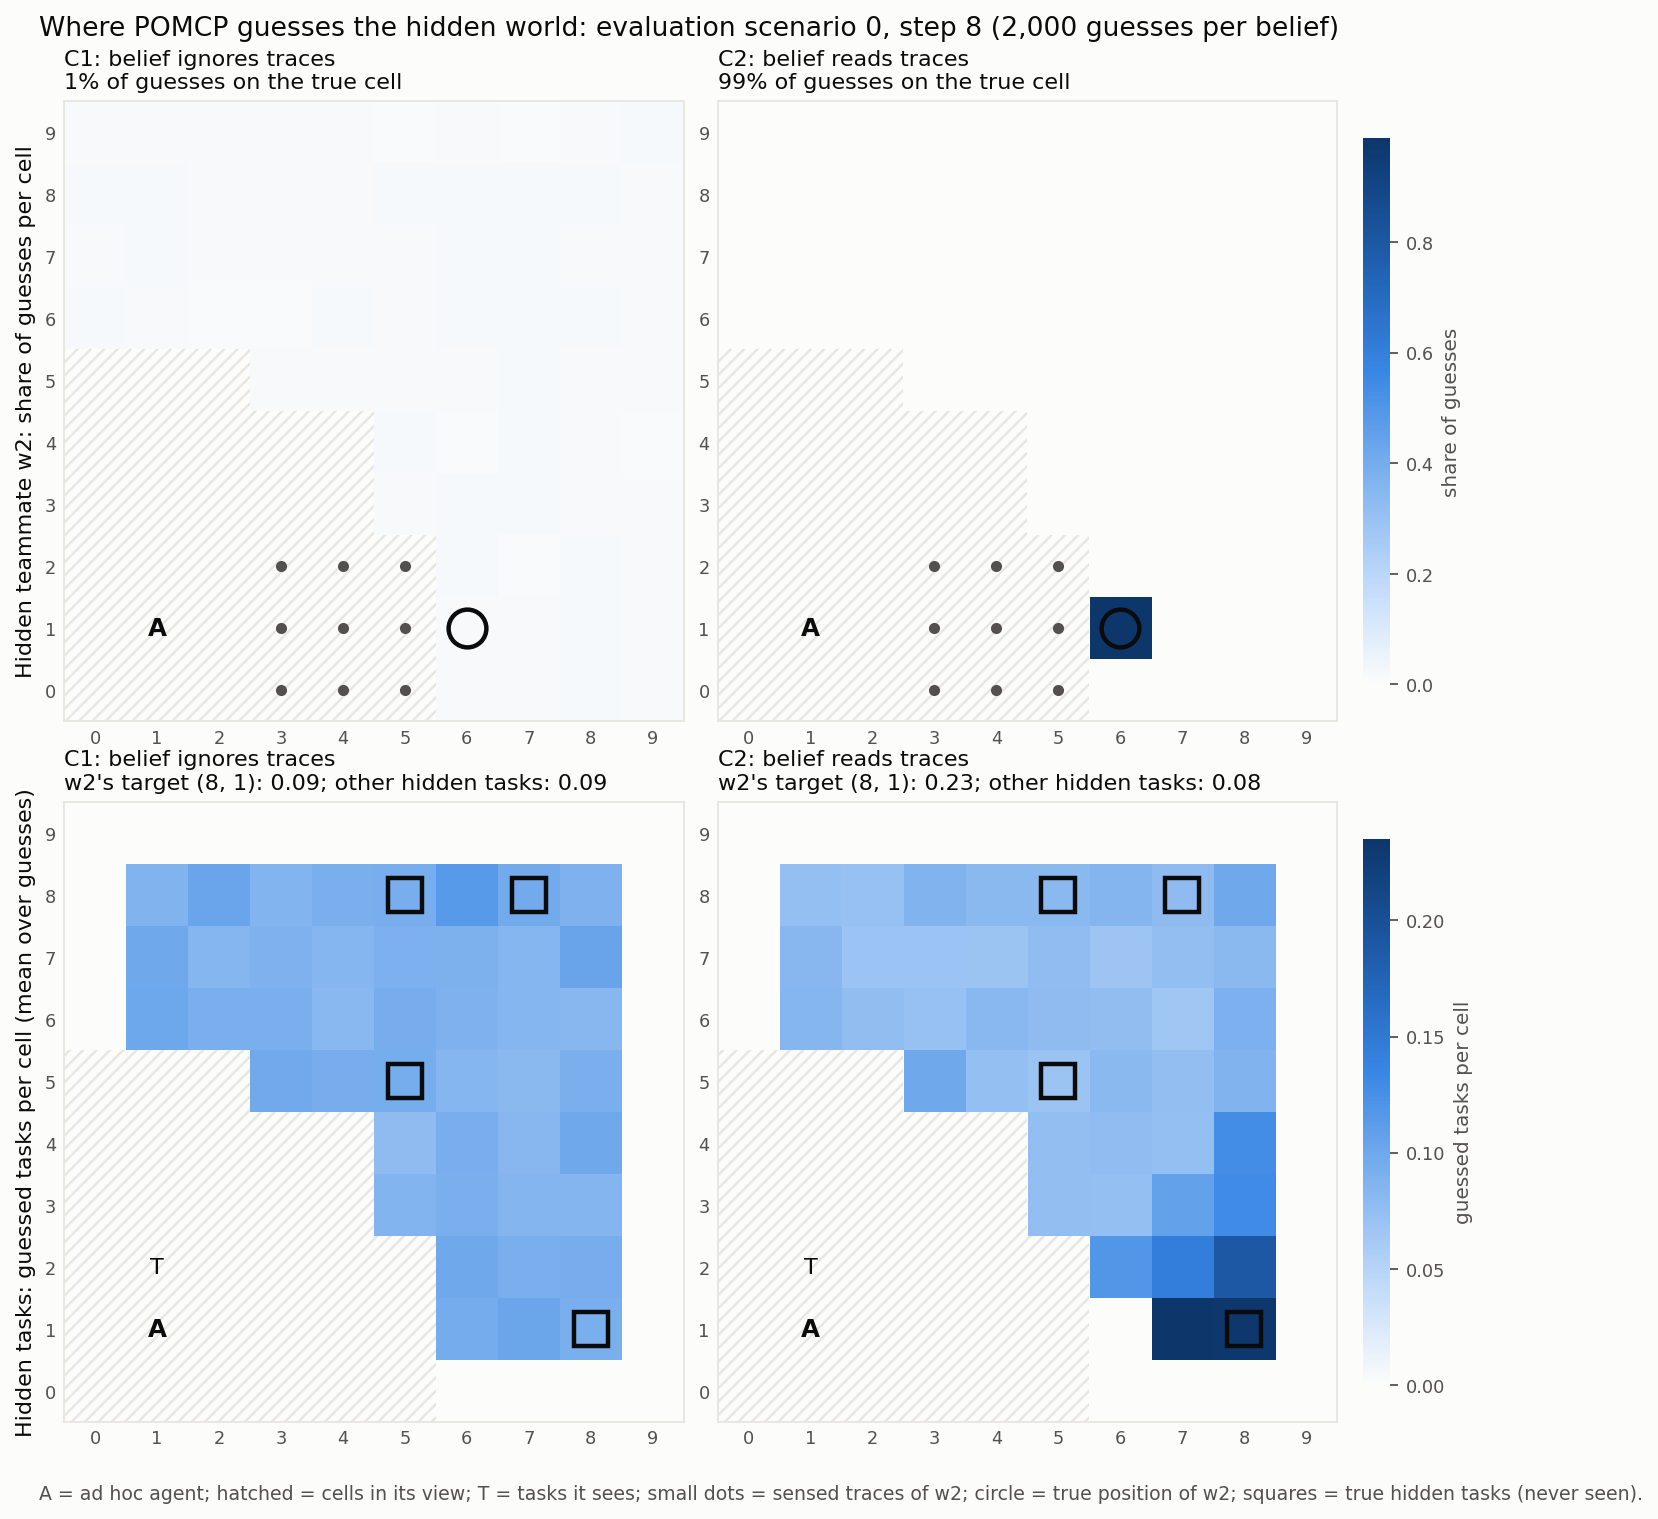
\includegraphics[width=0.95\linewidth]{../../results_analysis/Plots/pomcp_trace_belief.png}
  \caption{Where the beliefs put the hidden world (\file{results_analysis/demo_pomcp_traces.py --figure}). Cell shade =
  share of guesses (top) or guessed tasks per cell (bottom); hatched = cells in view; circle / squares = the truth.}
  \label{fig:belief}
\end{figure}

%=====================================================================================================================
\section{Experiment design}
\label{sec:design}
%=====================================================================================================================

All measurements use \file{results_analysis/evaluate_trace_pomcp.py} on the 100 shared hard evaluation scenarios
(\code{create\_evaluation\_set(100, task\_level\_range=(0.3, 1.5))}, seed 2026): intent traces, local sensing, ad hoc
level $0.9$ and view radius $0.25$, two teammates. Every episode seeds \code{random} and \code{numpy} with its scenario
index, so configurations face the same teammates' random choices as far as the play allows. Raw per-object and
per-episode rows are saved in \file{results_analysis/Results/trace_pomcp/}, so every number below can be recomputed with
\code{--summary}.

\subsection{Measurement 1: belief accuracy (\code{--belief})}

\paragraph{Question.} Do the guesses get closer to the truth when the belief reads traces?

\paragraph{Procedure.} In each scenario the ad hoc agent is driven by the cooperative teacher (\file{coop_expert.py}),
only so that the visited states are realistic; the teacher is not part of any belief. At each of the first 40 steps,
C1 and C2 each draw $50$ guesses from the \emph{same} observation, with the same random seed. The game's random state is
saved before and restored after measuring, so measuring does not change the game. For every hidden object:
\begin{itemize}[nosep]
  \item \textbf{hidden teammate} $j$ with true cell $p_j$: distance $=\frac1{50}\sum_{i}\lVert \hat p^{(i)}_j - p_j\rVert_1$
        and hit rate $=\frac1{50}\sum_i \mathbf 1[\hat p^{(i)}_j = p_j]$ over the guesses $i$;
  \item \textbf{hidden task} at true cell $q$: the distance from $q$ to the nearest guessed hidden task of each guess,
        averaged over guesses; hit rate = share of guesses with a guessed task exactly on $q$.
\end{itemize}
Rows are split by whether the agent sensed at least one trace of that teammate (for tasks: any bearing or help trace).

\paragraph{Statistics.} The difference C2 $-$ C1 is paired (same observation, same seed). Decisions within one game are
correlated, so the 95\% confidence interval is computed from the spread of the per-scenario mean differences
($1.96\cdot\mathrm{sd}/\sqrt{\#\text{scenarios}}$), not from the individual decisions.

\subsection{Measurement 2: games (\code{--games})}

\paragraph{Question.} Does POMCP play better when its belief reads traces?

\paragraph{Configurations.} C0, C1, C2 (Section~\ref{sec:beliefs}) at $0.1$ and $0.5$ seconds of search per decision,
and C1, C2 also at $2.0$\,s (added during the day to test whether a lack of search hides an effect),
\code{max\_depth=20} (about 10 steps ahead), $K=100$ particles, UCB constant $0.5$, discount $0.95$. C0 reuses its tree
between decisions, as in October. C1 and C2 start a new tree at every decision, so their belief is rebuilt from the
current traces (Section~\ref{sec:planning-world}).

\paragraph{Metrics} (per episode, 200-step cap): all tasks completed (yes/no), steps, timeouts, and the search effort
actually achieved: tree steps (\code{nsimulations}) and rollout steps per decision, and wall-clock seconds per decision.
Completion is reported with a Wilson 95\% interval,
\begin{equation}
  \frac{\hat p + \frac{z^2}{2n} \pm z\sqrt{\frac{\hat p(1-\hat p)}{n} + \frac{z^2}{4n^2}}}{1+\frac{z^2}{n}}, \qquad z=1.96,
\end{equation}
which behaves well near $0\%$ and $100\%$, where the usual $\hat p \pm z\sqrt{\hat p(1-\hat p)/n}$ fails.

\paragraph{The paired comparison C2 vs C1} (same scenario, same seed): the mean step difference over all scenarios
(timeouts count as 200), the mean step difference over scenarios both finish with a 95\% interval, the number of scenarios
where C2 is faster, slower or tied, and the number where only one of them finishes. Pairing removes the large differences
between scenarios (some need 20 steps, some 150), so a smaller effect becomes visible.

\paragraph{Running.} 18 worker processes in parallel (\code{--worker i --num-workers 18}), each running the
configurations one after another on its share of the scenarios. POMCP's budget is \emph{time}, so the amount of search
depends on machine load; the achieved search counts are therefore reported next to every result.

\paragraph{Why C2 vs C1, not C2 vs C0.} C1 and C2 have the same world, the same tree rules and the same cost per
imagined step. Only the belief differs. C0 differs in three ways at once (no hidden teammates, wrong task prior and count,
tree reuse), and its imagined steps are cheaper because it imagines fewer agents. C0 is a reference point, not a control.

%=====================================================================================================================
\section{Results}
\label{sec:results}
%=====================================================================================================================

All numbers come from \code{python3 results\_analysis/evaluate\_trace\_pomcp.py --summary} on the files in
\file{results_analysis/Results/trace_pomcp/} (commit \code{ab72bb9} plus the uncommitted changes of 20 November).

\subsection{Belief accuracy: traces carry a lot of information}

\begin{center}
\small
\setlength{\tabcolsep}{4pt}
\begin{tabular}{lp{2.6cm}rcc}
\toprule
Hidden object & Cases & $n$ & Distance C1 $\to$ C2 (cells) & Hit rate C1 $\to$ C2 \\
\midrule
teammate & a trace of it is sensed & 810 & $5.57 \to \mathbf{1.26}$ \ ($-4.31\pm0.20$) & $0.019 \to \mathbf{0.428}$ \ ($+0.41\pm0.04$)\\
teammate & no trace of it sensed & 766 & $5.57 \to 5.59$ \ ($+0.02\pm0.03$) & $0.017 \to 0.016$\\
teammate & all & 1{,}576 & $5.57 \to 3.36$ \ ($-2.21\pm0.20$) & $0.018 \to 0.228$\\
task & a bearing or help is sensed & 2{,}646 & $3.20 \to 2.90$ \ ($-0.30\pm0.11$) & $0.081 \to 0.130$ \ ($+0.05\pm0.02$)\\
task & none sensed & 529 & $2.29 \to 2.29$ & $0.084 \to 0.084$\\
\bottomrule
\end{tabular}
\end{center}
\setlength{\tabcolsep}{6pt}($n$ = hidden objects $\times$ decisions over 100 scenarios; $\pm$ = 95\% interval clustered by scenario.)

\paragraph{Reading.} When the agent senses a trace of a hidden teammate, reading it moves the guesses from ``anywhere out
of view'' (5.6 cells off, right 2\% of the time) to ``almost there'' (1.3 cells off, right 43\% of the time). When no
trace is sensed, C2 equals C1, as it must: this is the sanity check. Hidden tasks gain less: a bearing gives a direction
but no distance, and only some hidden tasks are anyone's target. Figure~\ref{fig:belief} shows one such moment.

\subsection{Games: the better belief does not (yet) give better play}

\begin{center}
\footnotesize\setlength{\tabcolsep}{3.5pt}
\begin{tabular}{lrcccccc}
\toprule
Config & $n$ & Completed [95\% CI] & Steps & Steps if done & Timeouts & Tree steps / dec. & Median s / dec. \\
\midrule
C0-0.1 & 100 & 89\% [81, 94] & 70.4 & 54.4 & 11 & 24 & 0.12 \\
C1-0.1 & 100 & 79\% [70, 86] & 87.1 & 57.1 & 21 & 8 & -- \\
C2-0.1 & 100 & 82\% [73, 88] & 86.0 & 61.0 & 18 & 7 & -- \\
C0-0.5 & 100 & 95\% [89, 98] & 43.4 & 35.2 & 5 & 203 & 0.53 \\
C1-0.5 & 100 & 89\% [81, 94] & 66.0 & 49.5 & 11 & 59 & 0.54 \\
C2-0.5 & 100 & 92\% [85, 96] & 71.1 & 59.9 & 8 & 68 & 0.54 \\
C1-2.0 & 100 & 94\% [88, 97] & 55.2 & 46.0 & 6 & 266 & 2.05 \\
C2-2.0 & 100 & 97\% [92, 99] & 54.1 & 49.6 & 3 & 363 & 2.05 \\
\bottomrule
\end{tabular}
\end{center}

\paragraph{Paired C2 vs C1} (same scenarios and seeds; step differences C2 $-$ C1 with 95\% intervals):
\begin{center}
\small
\begin{tabular}{lcccc}
\toprule
Budget & All scenarios & Both finish & C2 faster / slower / tied & Only C2 / only C1 finishes\\
\midrule
0.1 s & $-1.1 \pm 11.2$ & $-0.6\pm 8.4$ ($n=73$) & 35 / 30 / 8 & 9 / 6\\
0.5 s & $+5.0 \pm 9.4$ & $+7.6\pm 8.0$ ($n=86$) & 39 / 40 / 7 & 6 / 3\\
2.0 s & $-1.1 \pm 8.7$ & $+3.9\pm 6.3$ ($n=91$) & 35 / 46 / 10 & 6 / 3\\
\bottomrule
\end{tabular}
\end{center}

\paragraph{Reading.}
\begin{enumerate}[leftmargin=*]
  \item \textbf{No detectable trace effect on play.} At every budget the C2 $-$ C1 step difference is compatible with zero,
        and C2 finishes slightly more often (82/92/97\% vs 79/89/94\%), but every gap lies well inside the intervals.
        With 100 scenarios, effects smaller than about $\pm 8$ steps cannot be seen.
  \item \textbf{It is not only a lack of search.} At 2.0 s, C1 and C2 search more (266--363 tree steps per decision) than
        C0 at 0.5 s (203), yet they still play no better with traces. They also play worse than C0 (55 vs 43 steps).
  \item \textbf{A hypothesis for both observations: the teammate model.} In imagined steps, an untyped teammate gets a
        random heuristic (\code{l1}--\code{l6}), so POMCP's predictions of what teammates \emph{do} are poor. Putting
        teammates back into the belief (C1, C2) then makes imagination slower without making it right. Knowing
        \emph{where} a teammate is helps little if POMCP cannot predict \emph{what it will do}. This is a hypothesis, not a measurement; the test is to give C1/C2 the true
        teammate types and re-measure (Section~\ref{sec:next}).
  \item \textbf{C0 is the best player here}, but for reasons unrelated to traces: cheaper imagined steps (fewer agents)
        and tree reuse. It is a reference, not a control (Section~\ref{sec:design}).
\end{enumerate}

\subsection{Caveats}
\begin{itemize}[nosep]
  \item \textbf{The computer was suspended twice} during the runs (before 13:01 and 13:06--14:15, lid closed). Processes
        were paused, so game outcomes are valid. Only the decision in progress at the suspend lost search time, and the
        \emph{mean} seconds per decision are inflated (hence medians in the table; C0-0.5 mean 0.94, C2-2.0 mean 4.17).
        The 0.1 s C1/C2 medians are omitted because their wall time also includes drawing 100 fresh particles outside the
        search timer.
  \item \textbf{Run order favours C2.} Each worker ran C1 before C2. As workers finished, the remaining ones shared the
        CPU with fewer processes, so C2 got somewhat more search per decision (e.g.\ 363 vs 266 at 2.0 s). This bias
        favours C2, yet no effect appeared. Interleaving configurations would remove it.
  \item \textbf{One game per scenario and configuration}; the paired intervals already reflect scenario-to-scenario
        variation, but not seed-to-seed variation within a scenario.
  \item \textbf{C1 ignores memory} (Section~\ref{sec:beliefs}), so the belief gain is ``traces vs.\ nothing''.
  \item \textbf{Belief accuracy uses teacher-driven states}, not states POMCP itself visits; Rule constants were not
        tuned. Two C2-2.0 workers stopped without an error message (scenarios 90 and 93); those two games were rerun alone.
  \item \textbf{2.0 s was added during the day} (not in the plan) to test the ``too little search'' explanation.
\end{itemize}

\subsection{Answer to the instructor's question}

\emph{Can POMCP use traces, and be the teacher?} POMCP can use traces only once (i) its world carries them and (ii) its
belief reads them; neither was true in the original code. With the true trace meaning, its belief about hidden teammates
becomes much more accurate, so traces do carry a learnable ``language''. In this world, that better belief does not yet
translate into better play, and the evidence points at the teammate model rather than the traces. So C2 is a sound
\emph{ceiling for belief accuracy} today. Whether it is also a ceiling for \emph{play} depends on fixing the teammate model
first.

%=====================================================================================================================
\section{The teacher's new role and the next step}
\label{sec:next}
%=====================================================================================================================

\subsection{The teacher, old and new}

Until November the ``teacher'' was the hand-written cooperative expert (\file{coop_expert.py}). It saw the whole hidden
state, and a network was trained to copy its moves (behaviour cloning). That design drew both critiques: the student is
capped by a teacher whose competence is assumed, and copying moves is model-free learning.

In the new direction the teacher is \textbf{C2}: POMCP whose belief knows the true meaning of traces, the ``native
speaker'' of the instructor's analogy.
\begin{center}
\small
\begin{tabular}{p{3.6cm}p{5.2cm}p{5.6cm}}
\toprule
 & Old teacher (\code{coop\_expert}) & New teacher (C2) \\
\midrule
What it knows & the whole hidden state & only what the ad hoc agent senses (own view + traces); its one privilege is knowing what
  traces \emph{mean} \\
How it decides & hand-written rules, no lookahead & planning: imagines futures, maximises reward \\
Is its quality assumed? & yes & no: measured against C0/C1 (Section~\ref{sec:results}) \\
What the ad hoc agent learns from it & its moves (copying) & nothing is copied: the agent learns the trace meaning (a
  world model) and plans with it \\
\bottomrule
\end{tabular}
\end{center}
Its jobs: (1) the \textbf{ceiling} that a learned trace model is measured against; (2) \emph{not} a label source: the
learned model is trained on what really happened in logged episodes, so no teacher's competence is assumed; (3) later,
optionally, a planner whose search results train a prior network that makes search faster (Expert Iteration). The
\code{coop\_expert} remains as a baseline and a way to drive the agent when collecting data. The Gate~1 behaviour-cloning
student is shelved.

\subsection{Next step: C3, learning the language}

C2's rules (Section~\ref{sec:c2}) are the trace meaning written by hand. C3 must \emph{learn} it, without being told the
rules or the teammates' algorithms:
\begin{enumerate}[leftmargin=*]
  \item \textbf{Data.} Play many episodes in simulation (any ad hoc behaviour that visits varied states). At every step
        record what the agent senses (view + traces) and, \emph{in hindsight}, the truth: the cells of hidden teammates and
        hidden tasks. Learning from the truth in logged experience is learning a world model. No teacher is involved.
  \item \textbf{Model.} A small network $q_\phi(\text{hidden cell} \mid \text{sensed traces, view})$ that outputs, for each
        teammate, a probability for every grid cell (and a map for hidden tasks). It is trained by maximum likelihood
        (cross-entropy) on the recorded truth. It is the learned counterpart of \code{read\_traces} + Rules 1--3.
  \item \textbf{Plug-in.} C3 = C1 whose \code{\_place\_hidden\_teammate} (and task proposals) draw from $q_\phi$ instead of
        the hand-written rules. POMCP itself does not change.
  \item \textbf{Score.} Measurement 1 (belief accuracy) and Measurement 2 (games), reported as the share of the
        C1 $\to$ C2 gap that C3 closes: ``C3 recovers $X\%$ of the benefit of knowing the language''.
\end{enumerate}
A more principled alternative learns the forward observation model $P(\text{traces}\mid\text{state, history})$ and
weights particles with it, Eq.~\eqref{eq:bayes}. It needs particles that carry their recent history, so it is kept for
later.

\subsection{Other open items}
\begin{itemize}[nosep]
  \item \textbf{First: the teammate-model test} (Section~\ref{sec:results}): rerun C1 and C2 with the teammates' true
        types in imagination. If C2 then beats C1, traces pay off once teammates are predicted well, and C3 should learn
        both where teammates are and how they act.
  \item \textbf{C1 + memory control}: place hidden teammates near where they were last seen, to separate what traces add
        beyond the agent's own memory (Section~\ref{sec:beliefs}).
  \item \textbf{Teammate behaviour}: in imagined steps, an untyped teammate gets a random heuristic (\code{l1}--\code{l6}).
        A standing help trace says ``this teammate keeps trying to load here'', which a learned model could also use to
        predict teammates.
  \item \textbf{Search cost}: imagining the whole team makes each imagined step expensive, so at a small budget C1/C2
        search much less than C0. Remedies: a larger budget, cheaper teammate models, or a prior network (Expert
        Iteration).
  \item \textbf{Harder settings}: a larger grid, a smaller view or more teammates make hidden information matter more,
        giving traces more room to help.
  \item \textbf{Trace matching in the tree}: comparing coarse trace summaries in \code{observation\_is\_equal}, so that
        the tree also branches on what traces the agent will see next (value of information).
\end{itemize}

%=====================================================================================================================
\section{Source map}
\label{sec:source-map}
%=====================================================================================================================

Files are relative to the repository root. ``Framework'' files belong to AdLeap-MAS and are used, never modified.

\begin{center}
\small
\begin{tabular}{p{5.2cm}p{7.3cm}l}
\toprule
File / function & What it implements & Section \\
\midrule
\file{src/envs/LevelForagingEnv.py} (framework) & LBF world: transition, loading~\eqref{eq:load}, visibility,
  \code{environment\_transformation}, \code{sample\_state} & \ref{sec:setting} \\
\file{src/communication/traces.py}: \code{TraceField} & trace storage; \code{decay}, \code{emit}, \code{fusion},
  \code{diffuse} & \ref{sec:traces} \\
\file{src/envs/StigmergicLevelForagingEnv.py}: \code{StigmergicLevelForagingEnv} & the real game: world step + trace
  update + the agent's observation tensor & \ref{sec:traces} \\
\quad\code{emit\_intent\_traces} & emission rules \eqref{eq:help}, \eqref{eq:bearing} (shared with the planning world) &
  \ref{sec:traces} \\
\quad\code{bearing\_to\_target} & bearing \eqref{eq:bearing} & \ref{sec:traces} \\
\file{src/utils/tensor_convert.py}: \code{dict\_to\_tensor} & local trace sensing (visibility mask) & \ref{sec:traces} \\
\file{src/utils/find_visible.py}: \code{find\_visible\_grids} & visible cells $V_t$ & \ref{sec:setting} \\
\file{src/utils/scenarios.py}: \code{make\_scenario} & scenario generation (ad hoc level/view, task levels) &
  \ref{sec:setting} \\
\file{src/reasoning/pomcp.py} (framework): \code{pomcp\_planning}, \code{POMCP.planning/search/simulate/rollout} &
  POMCP & \ref{sec:pomcp} \\
\file{src/reasoning/node.py} (framework): \code{find\_new\_PO\_root}, \code{particle\_revigoration} & tree reuse,
  particles & \ref{sec:pomcp} \\
\file{src/reasoning/qlearn.py} (framework): \code{ucb\_select\_action} & UCB, Eq.~\eqref{eq:ucb} & \ref{sec:pomcp} \\
\file{src/communication/traces.py}: \code{TraceField.copy} & independent trace copy for imagined worlds &
  \ref{sec:planning-world} \\
\file{src/envs/TracePlanningEnv.py}: \code{TracePlanningEnv} & POMCP's world with traces: \code{from\_real},
  \code{copy}, \code{step}, \code{sample\_state} & \ref{sec:planning-world} \\
\quad\code{sample\_state}, \code{\_sample\_corrected}, \code{\_place\_hidden\_teammate} & belief samplers C1 (and C2)
  & \ref{sec:beliefs} \\
\quad\code{read\_traces} & C2's decoder: youngest trace, steps, radius, bearings, help & \ref{sec:c2} \\
\quad\code{cosine}, \code{neighbours}, \code{on\_border} & helpers for Rules 1--3 and the generator rules &
  \ref{sec:beliefs} \\
\quad\code{infer\_emitted} & emitted vs.\ diffused sensed traces, Eq.~\eqref{eq:diffused-test} & \ref{sec:planning-world} \\
\file{src/utils/evaluation.py}: \code{run\_episode}, \code{run\_pomcp\_episode} & one episode with any policy / with POMCP
  (C0, or a \code{TracePlanningEnv} belief) & \ref{sec:planning-world} \\
\file{results_analysis/demo_pomcp_traces.py} & the breakpoint demo & \ref{sec:observation-model} \\
\file{tests/test_trace_planning_env.py} & tests of the planning world and the beliefs & \ref{sec:planning-world}, \ref{sec:beliefs} \\
\bottomrule
\end{tabular}
\end{center}

\end{document}
